\documentclass[11pt]{article}
\usepackage{amsmath,amsthm,verbatim,amssymb,amsfonts,amscd, graphicx}
\usepackage{graphicx}
\usepackage{subcaption}
\usepackage{listings}
\usepackage{float}
\usepackage{url}
\usepackage{titlesec}
\setcounter{secnumdepth}{4}


\graphicspath{{./times/}}
\topmargin0.0cm
\headheight0.0cm
\headsep0.0cm
\oddsidemargin0.0cm
\textheight23.0cm
\textwidth16.5cm
\footskip1.0cm

\titleformat{\paragraph}
{\normalfont\normalsize\bfseries}{\theparagraph}{1em}{}
\titlespacing*{\paragraph}
{0pt}{3.25ex plus 1ex minus .2ex}{1.5ex plus .2ex}


\begin{document}
\title{CS 5220\\ Comparative Studies on the Computational Speed Between Skylines and Pardiso Sparse Direct Solver}
\author{Marc Aurele Gilles (mtg79)\\ Wenjia Gu (wg233)\\Wensi Wu(382) }
\maketitle

\section{Introduction}\label{sec:intro}

The goal of this project was to compare the performance of two different sparse direct solvers. First, we took a look at our in-house quasi-static structural code, $3D\_geom\_nonlin\_truss.c$. The numerical implementation of the code is described in section \ref{sec:method}.  The $3D\_geom\_nonlin\_truss.c $ is a geometrically nonlinear finite element code embedded with the feature of analyzing truss structures using skyline indexing scheme and Cholesky-like factorization to solve a large system of equations. In section \ref{sec:setup}, we describe the two different input structures we used for the performance analysis.  A detailed description of the skyline indexing scheme is provided in section \ref{sec:originalCode}. \\

The solver in which we compared our original code with is a MKL sparse direct solver: Pardiso. Pardiso has features of solving large symmetric and nonsymmetric linear systems of equaitons, $AX=B$, using parallel $LU$, $LDL^T$ or $LL^T$ factorization where $L$, $U$, and $D$ are the low triangle, upper triangle and the diagonal of matrix $A$ respectively. The solver employes parallel pivoting methods based on OpenMP directives, which result in the robust and memory-efficient performance. In section ~\ref{sec:newCode} we will describe how we translated the skyline indexing scheme in the original code into Compressed Sparse Row (CSR) format in order to take advantage of the Pardiso solver.\\

After we successfully hooked Pardiso into our original code, we conducted weak and strong scaling studies for both sparse direct methods. The results can be found in section \ref{sec:scaling}.  


\section{Numerical Method}\label{sec:method}

The numerical analysis of truss problems can be written in the form:
$$F_l(u)=0$$
u is the displacement, F is a system of $n$ non-linear equations where n depends on the number of nodes and degrees of freedom, and l is the maximum load factor.\\

We solve this system of non-linear equation using an iterative method, starting at $l=0$, and incrementally increasing $l$ until it reaches the user specified maximum $l^{\star}$. Each $F_l(u)=0$ equation is solved using the Newton Raphson iteration method. In other words, we repeatedly solve the system equation $F_l(u_{t+1}) \simeq F_l(u_t) + K_l(u_t)*u_{t+1}$ until the solution converges to a defined tolerance close to 0. $K_l(u_t)$ is the Jacobian matrix at $u_t$, which in this problem is the same as the Stiffness matrix. Each iteration is essentially a linear solve:
$$K_l(u_t)*u_{t+1}=-F_l(u_t)$$.

\section{Initial Profile Result}\label{sec:profiling}

\subsection{Timing}
To identify the bottleneck of our original code, we ran the code with a test case, a pyramid made of 59700 nodes and 20100 elements, using amplxe. This case gave us a stiffness matrix size of 39800 * 39800. The CPU time spent in executing the orginal code is show in the table below. As shown, majority of the computation time is spent on the linear solve section due to dimension of the matrix. Although the size of stiffness matrix is very large, we noticed that it is actually very sparse. Hence, implementing a sparse solver would be our primary approach to speed up the code. \\

Below is the timing results of the original code:

\begin{center}
	\begin{tabular}{||c c c ||} 
		\hline
		Function & Description & CPU Time \\ [0.5ex] 
		\hline\hline
		solve & Sparse linear solve & 32.560s  \\ 
		\hline
		intel memset  & allocates memory & 0.273s  \\
		\hline
		printf fp & prints to file & 0.132s  \\
		\hline
		stiff & computes stiffness matrix & 0.104s  \\
		\hline
		forces & computes residual forces & 0.078s  \\[1ex] 
		\hline
	\end{tabular}
\end{center}

\subsection{Vectorizaiton}
On top of introducing sparse direct solver to the original code, we looked into how efficient the vectorization of the solve function is. As shown in the vectorization report (see figure 1 \ref{fig:vectorization}), the solve function shows some vectorization, which increases the speedup of the main loop by a factor of 1.75. 

\begin{figure}[h]
	\begin{center}
		
		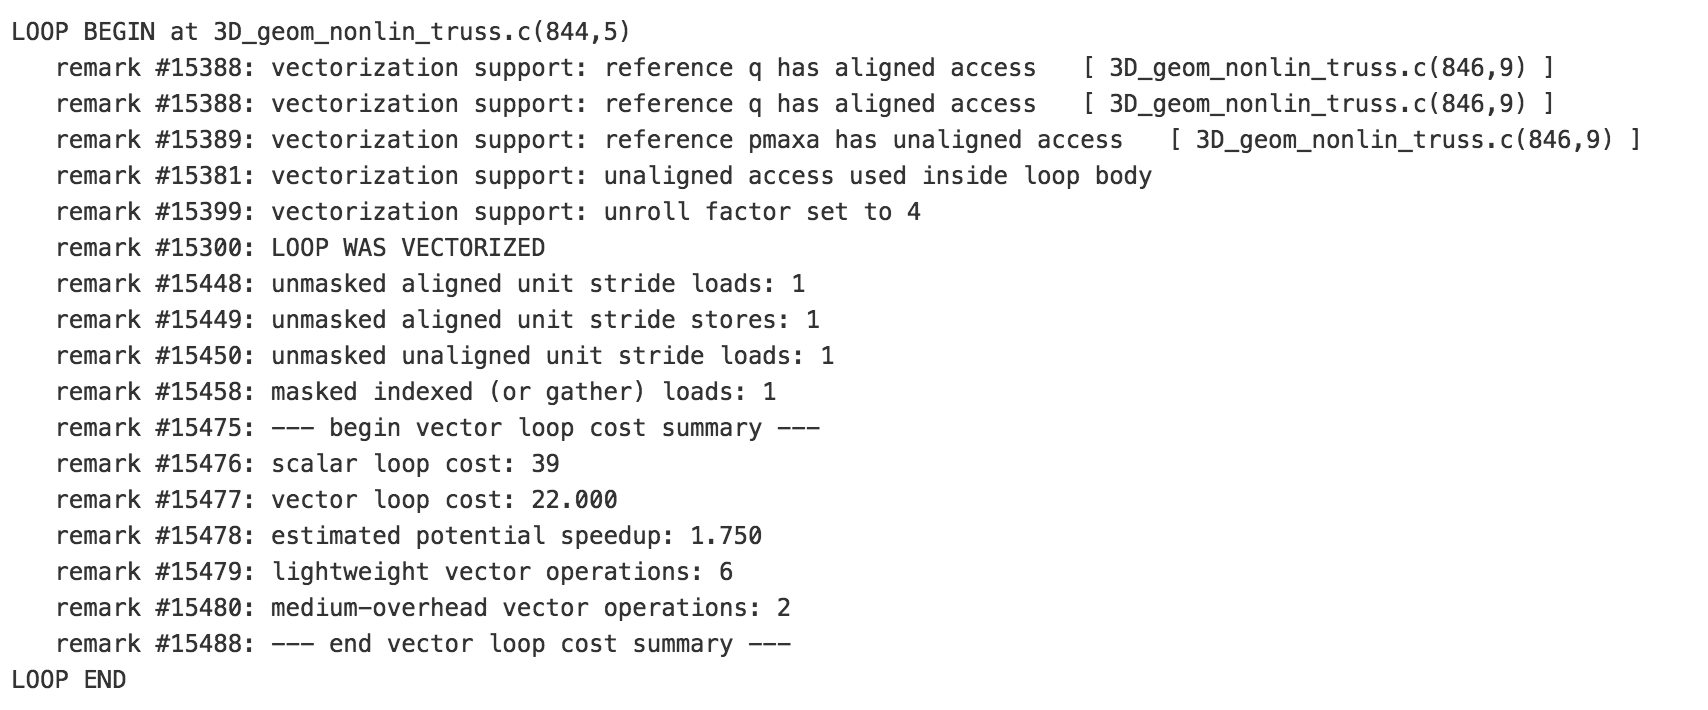
\includegraphics[width=11cm]{vectorization}
		\caption{Vectorization report of the solve function}
		\label{fig:vectorization}
	\end{center}
	
\end{figure}

\section{Setup: generating input structures}\label{sec:setup}

Since our objective is to speed up computation time and conduct scaling studies, we need to be able to generate input structures of variable sizes.\\

We wrote two scripts that generate two different type of input structures, a Warren truss bridge (see figure ~\ref{fig:chain}) , and a "pyramid" structure (see figure ~\ref{fig:pyramid}) .


\begin{figure}[h]
\begin{center}

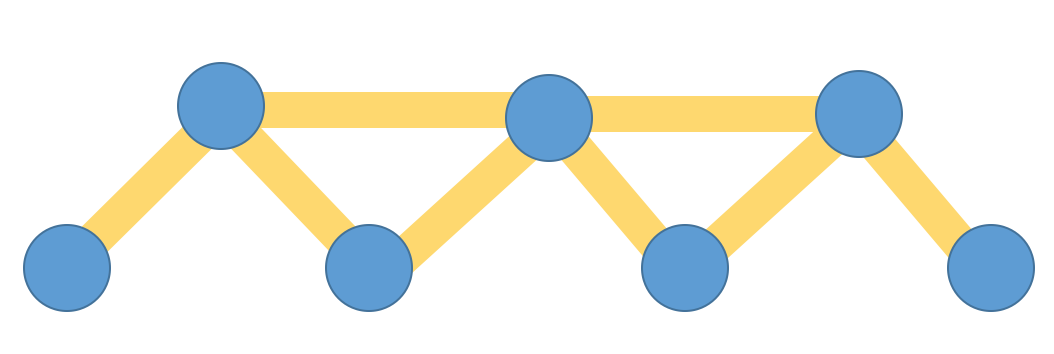
\includegraphics[width=8cm]{chain}
\caption{A Warren truss bridge of 7 elements}
\label{fig:chain}
The blue circles are the nodes, and the yellow bars are the elements
\end{center}

\end{figure}


\begin{figure}[h]
\begin{center}

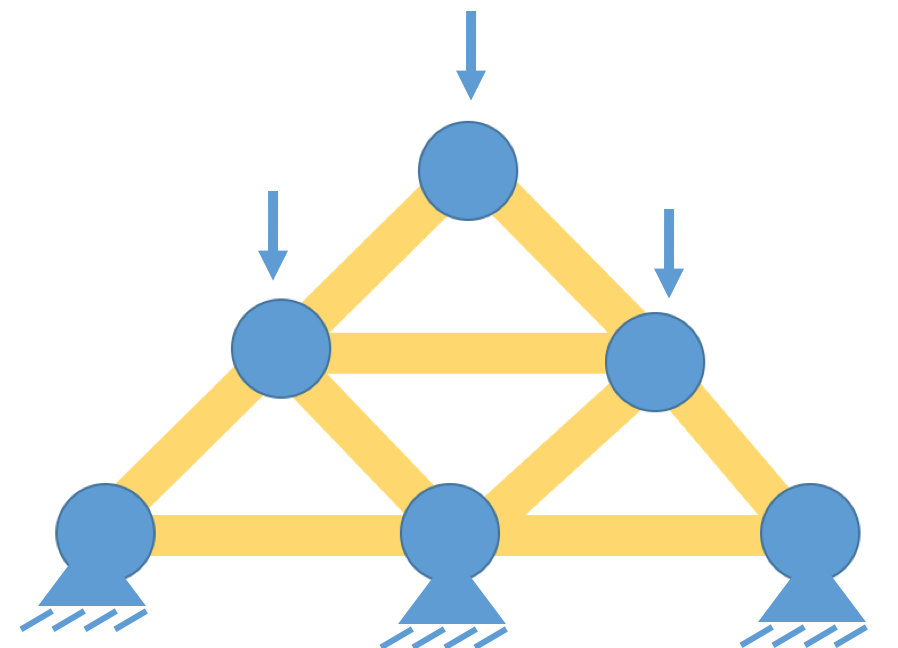
\includegraphics[width=8cm]{pyramid}
\caption{A pyramid structure of 6 elements}
\label{fig:pyramid}
The blue circles are the nodes, and the yellow bars are the elements
\end{center}

\end{figure}


For each structure we declare the position of each node, the position of each elements (as defined by a pair of nodes), the properties of each element (cross section area and the corresponding young's modulus), and an applied load on each node. For the Warren truss bridge, the first base node was constrianted with fixed support and the last base node was constrained with roller support. We applied a load to every other node at the top of truss. For the pyramid structure, all base nodes were constrained with fixed support. We applied a load to all boundary nodes.\\

These two different structure give rise to significantly different running time and sparsity patterns in the stiffness matrix, for a fixed number of elements. Indeed, the truss structure produces a stiffness matrix with a small dense band, which is not the case for the pyramid structure.

\begin{figure}[H]
\begin{center}
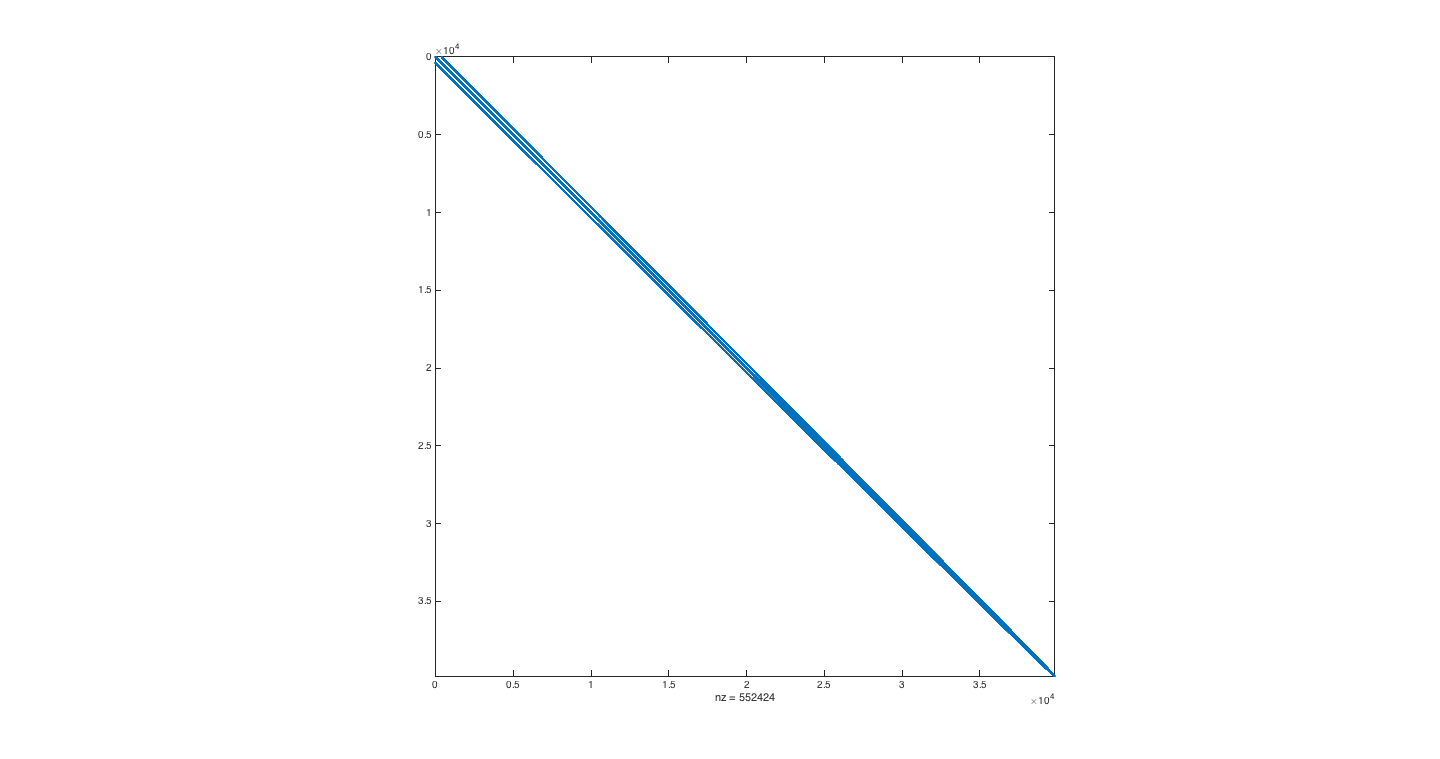
\includegraphics[width=15cm]{pyramid-sparsity.png}
\caption{Sparsity structure of the stiffness matrix generated from the pyramid structure}
\label{fig:pyramid-sparsity}
\end{center}

\end{figure}

\section{Original code}\label{sec:originalCode}
The original code reads in all of the parameter of the structure, and performs numerical method described in section \ref{sec:method}. At each iteration generates a stiffness matrix (the Jacobian), and uses a linear solve that takes advantage of the sparsity pattern of the matrix. The matrix storage format is Skyline indexing (described below). The solver takes advantage of the regular access of the skyline indexing to perform a fast Cholesky-like factorization of the form $LDL^T$. In addition, the original code is running in serial.


\subsection{Skyline}
Skyline is a sparse indexing format widely used in finite element codes for structural mechanics. Note that the term "Skyline" also refers to the set of entries from first non-zero to the diagonal in each column. A matrix in skyline format is three arrays: 
\begin{enumerate}

\item value array: an array contains the values in the stiffness matrix between the first non-zero entry of each column and the diagonal
\item MAXA array: a  pointer array stores the index of the diagonal values in the SS array; the last element is the size of the value array +1 in case of the fortran-style indexing.
\item KHT arrary: an array defines the number of entries from first non-zero value of each column to the diagonal of the stiffness matrix; the first element is default to 1. 
\end{enumerate}

\begin{figure}[h]
\begin{center}

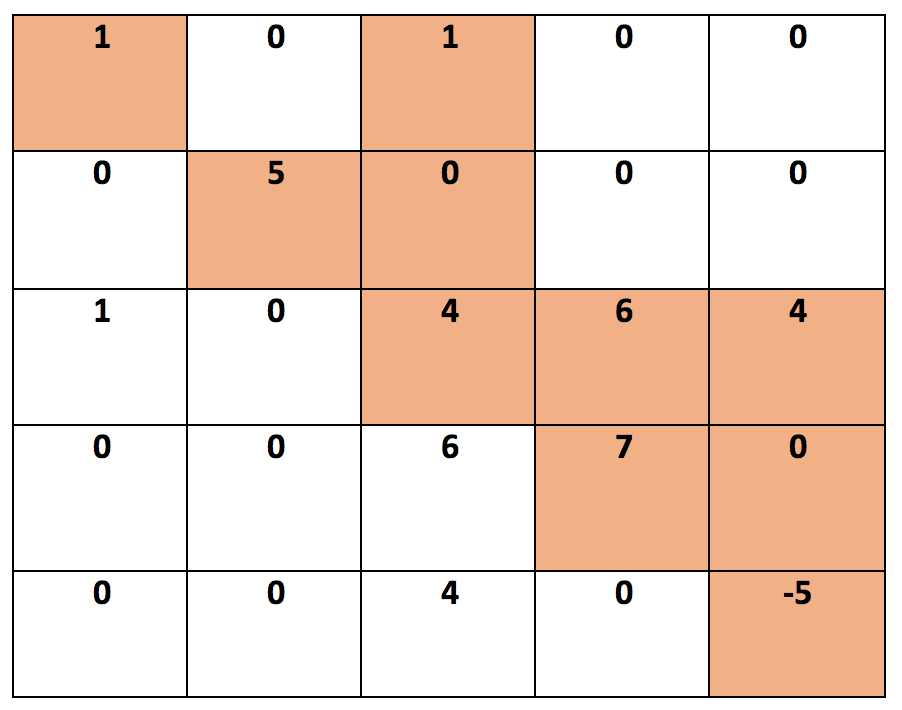
\includegraphics[width=8cm]{skyline}
\label{fig:skyline}\\
\caption{Example of a matrix stored in skyline format}
The entries in orange are the values stored in skyline arrays
\end{center}

\end{figure}
The matrix above in skyline format would be:

\begin{align}
values&=[1, 5, 4, 0, 1, 7, 6, -5, 0, 6]\\
MAXA&= [1, 2, 3, 6, 8, 11] \\
KHT&=[1, 0, 2, 1, 2]
\end{align}

 The skyline indexing takes advantage of the fact that matrices that arise in this field are usually banded, symmetric positive definite matrices. Solving the system with such a matrix is usually (like in our code) by doing a sparse Cholesky-like decomposition. See \cite{Bathe} for details. One reason that makes the skyline indexing attractive is that the fill happening during the decomposition is only within the "skyline".\\
 
Though the skyline format is usually very efficient for small systems, it is known that the format can be less than ideal in bigger systems, where the "band" of the matrix grows large, and becomes itself  sparse.

\section{Optimized code}\label{sec:newCode}
To optimize the original code, we translated the skyline format into a Compressed Sparse Row format and then used the MKL parallel sparse solver: Pardiso.

\subsection{Compressed sparse row}

Compressed Sparse Row (CSR) format is the most common sparse indexing format in scientific computing. A matrix in CSR format constitutes of three arrays:
\begin{enumerate}
\item the value array which contains the non-zero elements of the matrix
\item the column pointer array, where element i is the number of the column in A that contains the i-th value in the values array
\item the row array, where the element j of this integer array gives the index of the element in the values array that is first non-zero element in a row j of A
\end{enumerate}
Note that since pardiso a symmetric solver, we only need to solve the upper triangular part of the matrix
\begin{figure}[H]
\begin{center}

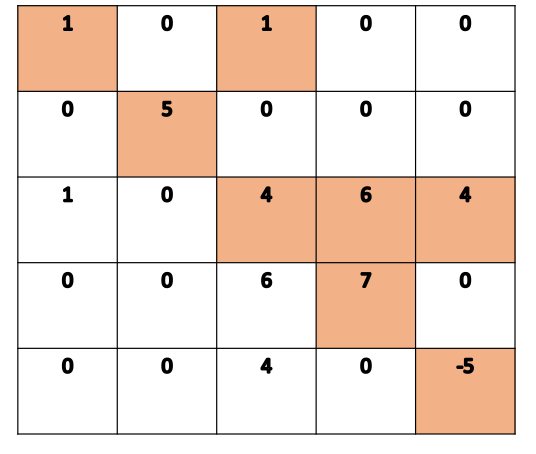
\includegraphics[width=8cm]{csr}
\label{fig:csr}\\
\caption{Example of a matrix stored in CSR format}
The entries in orange are the entries saved in the symmetric CSR format
\end{center}
\end{figure}

The matrix above in skyline format would be:

\begin{align}
values&=[1,1,5,4,6,4,7,-5]\\
columns&= [1,3,2,3,4,5,4,5] \\
rows&= [1,3,4,7,8,9] 
\end{align}

\subsection{Pardiso}
Pardiso is the sparse solver of the library MKL. It can solve many different types of sparse systems such as real or complex, symmytric, structurally symmertric or non-symmetric, definite or indefinite. See \cite{Intel} for details. In our case, the stiffness matrix is real symmetric positive definite. Pardiso has a wealth of different settings to change pivoting strategies, number of threads, number of iterative refinement steps, etc. In our case, pardiso performs a factorization of the form $LL^T$, uses the parallel version of the nested dissectin algorithm and takes 2 refinement steps. 

\subsection{Timing comparisons}
Figure \ref{fig:chaincomp} shows the comparisons of running time between the original solver and the pardiso solver using single thread  on the truss structure. \\

We observe that on the truess structure, both solver are very fast (about 1 second for a structure with 30.000 elements, but the original solver is slightly better. This is likely due to the fact that the original solver is very efficient on this system generated by the structure. Indeed as observed earlier the stiffness matrix in this case have a small but dense band, which is where the solver using the skyline format excels.


\begin{figure}[H]
\begin{center}

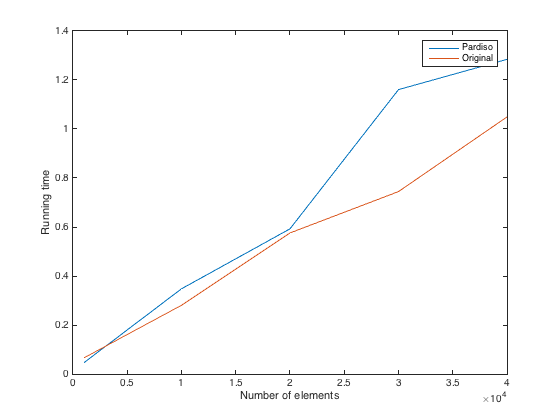
\includegraphics[width=10cm]{chainplot}
\caption{Comparison of running time on truss structures}
\label{fig:chaincomp}
\end{center}
\end{figure}

Figure \ref{fig:pyr_comp} shows the comparisons of running time between the original solver and the pardiso solver using single thread on the pyramid structure. \\

Contrary to the truss structure, the pardiso solver is much faster on the pyramid structure. This is likely due to the fact that the skyline format keeps a very high number of zeros, and therefore performs a lot of unnecessary arithmetic. Indeed, for the case where we have a 40.000, over $98\%$ of the entries saved by the skyline format are zeros.


\begin{figure}[H]
\begin{center}

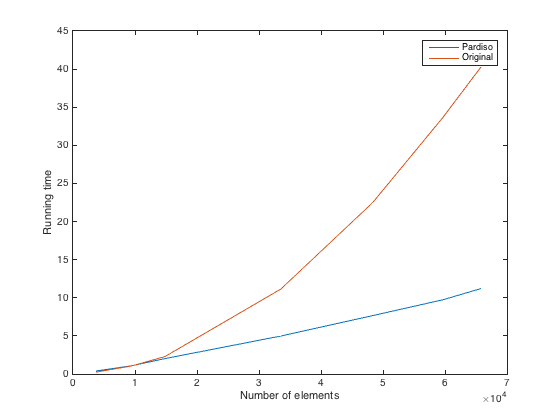
\includegraphics[width=10cm]{pyrplot}
\caption{Comparison of running time on pyramid structures}
\label{fig:pyr_comp}
\end{center}
\end{figure}


\section{Scaling studies}\label{sec:scaling}
The base case considered here is the original finite element code embedded with skyline indexing scheme and Cholesky factorization method. We are comparing the base case with a optimized case where the skyline indexing scheme was replaced by CSR and the Cholesky factorization solve was replaced by Pardiso solver. 

\subsection{Strong scaling}
We performed a strong scaling studying of the optimaized code on a pyramid structure containing 59700 elements (which corresponds to a base of 200 nodes). This gave us a problem size of n = 39800 where n is the size of the stiffness matrix. Figure \ref{fig:strongplot} shows a plot of running time against the number of threads used. We fixed the number of OpenMP thread to 1 and consider the range of processors from 1 to 12. Firgure \ref{fig:speedupstrong} shows the speedup against the number of threads used. We measured speedup as the ratio of the CPU time spent on solving the linear system of equation for the base case verse the CPU time spent on solving the linear system of equation for the optimatized case. We observe that the speed up is relatively small, approximately 1.5 when 5 threads were used and no additional speedup is attained by increasing the number of threads used. \\

\begin{figure}[H]
	\begin{center}
		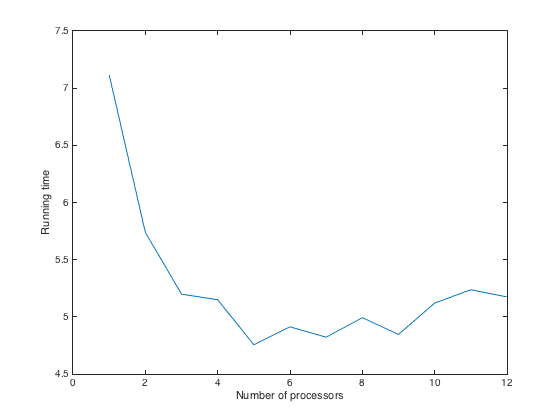
\includegraphics[width=11cm]{strongplot}
		\caption{Fixing number of OpenMP thread = 1, and varying the number of processors from 1 to 12}
		\label{fig:strongplot}
	\end{center}
\end{figure}

\begin{figure}[H]
	\begin{center}
		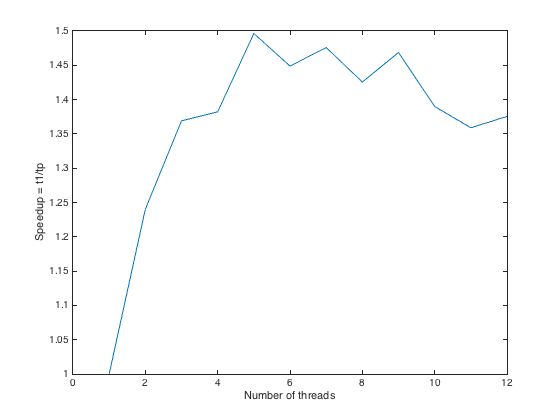
\includegraphics[width=11cm]{speedupstrong}
		\caption{Speedup ratio vs. varying the number of OpenMP threads from 1 to 12 }
		\label{fig:speedupstrong}
	\end{center}
\end{figure}

\subsection{Weak scaling}
We performed a weak scaling study for the optimized code on the pyramid structure. We fixed the number of processor to 1 and consider the range of 1 to 12 threads. On figure 8, we observed that the pardiso solver exhibits a linear growth in running time as the number of element increases, therefore we increase the number of threads linearly with the number of elements. Figure \ref{fig:weakplot} shows the result of the weak scaling study. We observe that the running time increases as the number of thread increases. This is expected as the strong scaling study revealed that the speedup on fixed size is not significant. These results suggests that using the right solver for the specific structure has a lot more impact on the running time than a solver than running in parallel.

\begin{figure}[H]
	\begin{center}
		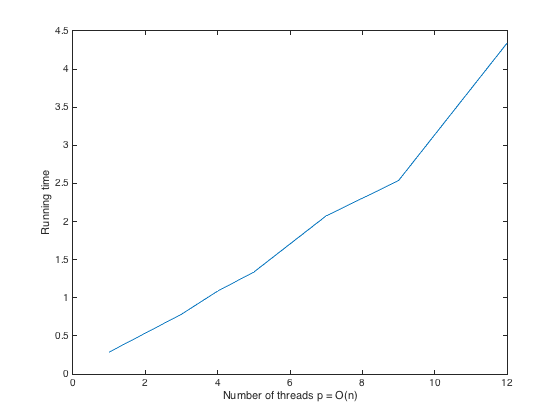
\includegraphics[width=11cm]{weakplot}
		\caption{Fixing number of processor = 1, and varying the number of OpenMP threads from 1 to 12 }
		\label{fig:weakplot}
	\end{center}
\end{figure}

\section{Conclusion}\label{sec:conclusion}
We compared the performance of two direct solvers: a solver that's popular in the field of structural mechanics, and an all purpose sparse direct linear solver: pardiso. We found that their performance depended heavily on the structure used, and that pardiso scales much better for structures that give rise to stiffness matrix having large, sparse bands. We then performed a scaling studies on the code that uses the pardiso solver, and found that limited speed was achieved by increasing the number of threads used. 

\section{Future Work}\label{sec:future}
It would be interesting to try different structures and different solvers. In particular, if we had more time, we would compare these two solvers to an iterative solver. An interesting question would then be to determine if solving each Newton step approximately (i.e. taking only a small number of steps in the iterative linear solver), but performing more Newton step would lead to speedup. 

\begin{thebibliography}{2}
	\bibitem{Bathe} Bathe, K., Wilson, E. \emph{Numerical methods in finite elment analysis}. Englewood Cliffs, N.J.: Prentice-Hall., 1956.
	\bibitem{Intel} Intel MKL PARDISO - Parallel Direct Sparse Solver Interface\\
	 https:// software.intel.con/en-us/node/470282
\end{thebibliography}

\end{document}